\section{Results}
% prec:0.154787009701     f1:0.179024390244       jac:0.0983123493169

We performed an experiment to evaluate the performance of the feature classification. The experimental setup described in the previous section shows that we have many parameters that could influence the classification performance. We will therefore first show results for a certain set of parameters that performed well. In the further sections, we explore the effects of different parameters, such as different images, classification algorithms of feature parameters.

%In this case, the classifiers were trained on section two and three and tested on section one. Furthermore, these results were obtained using synthetic oversampling using the SMOTE method.


\begin{figure}
	\centering
	\begin{tabular}{cc}
		\subfloat{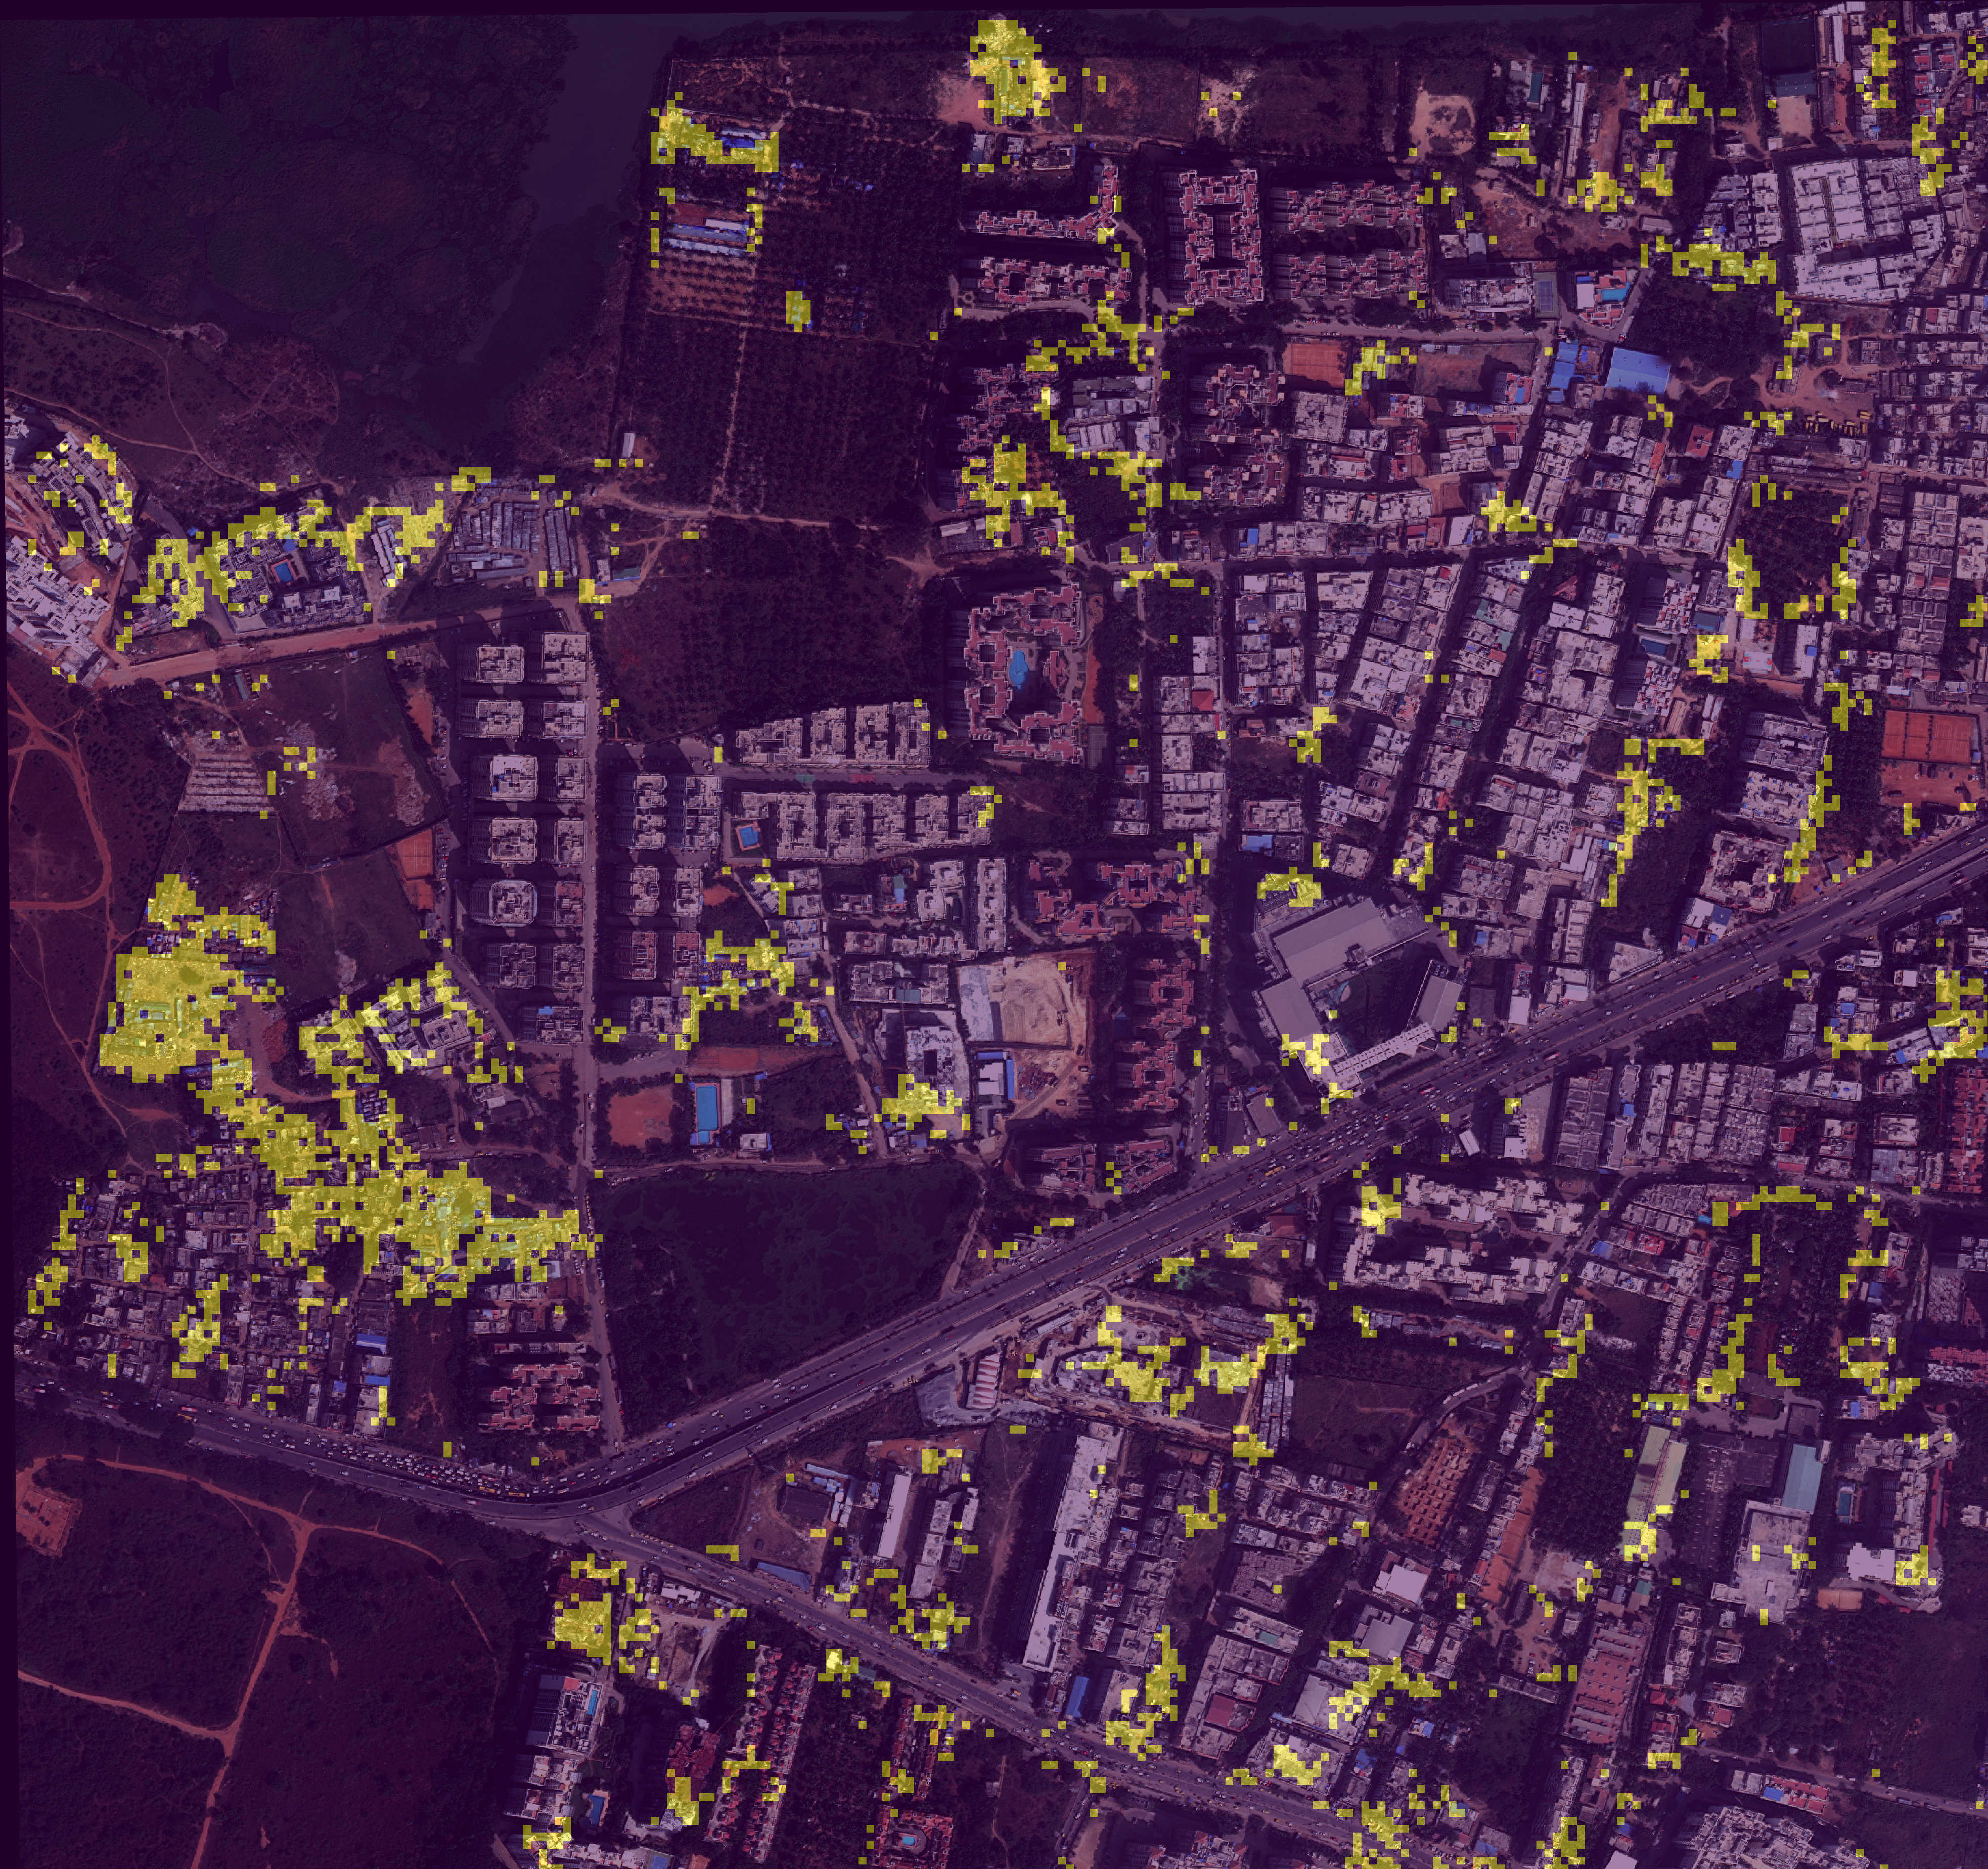
\includegraphics[width=7cm]{images/BestOverlay}}&
		\subfloat{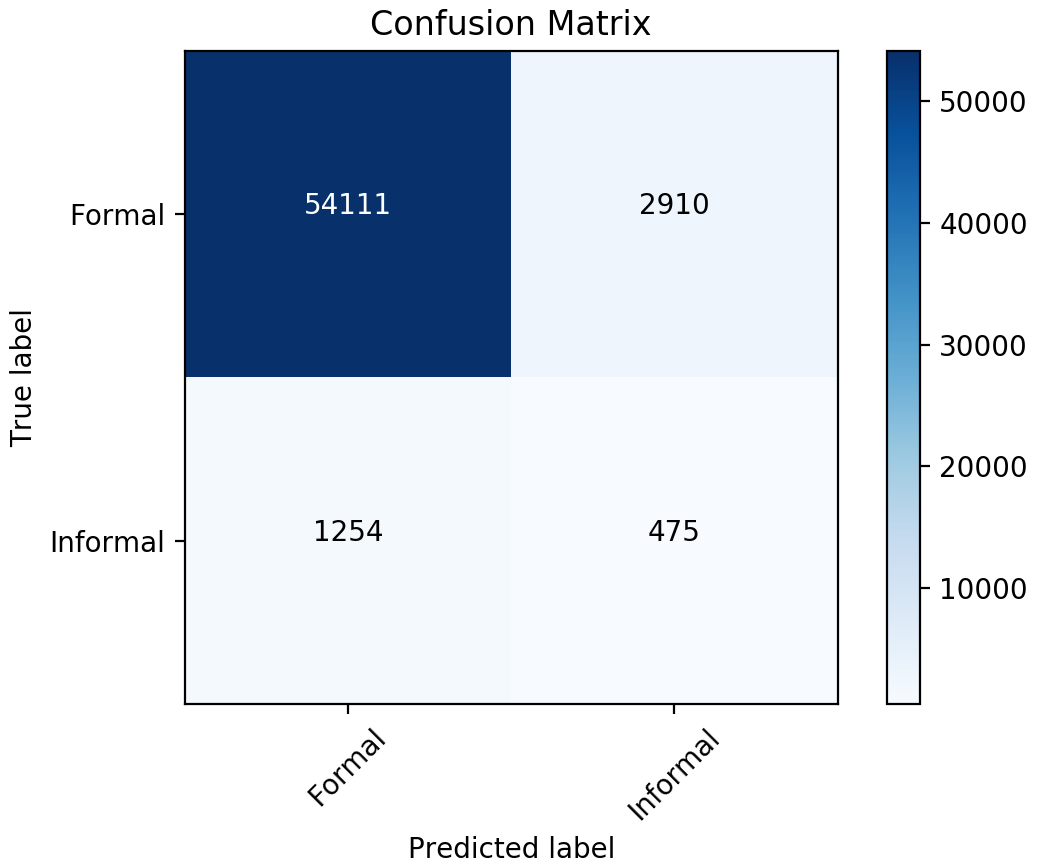
\includegraphics[height=7cm]{images/BestConfusion}}
	\end{tabular}
	\caption{Classification of Section 2 using Gradient Boosting}
	\label{fig:res_best}
\end{figure}

Figure \ref{fig:res_best} shows the most fitting classification we could achieve using our current features and classifiers. The results are produced by the experiment described in the experimental setup. For this specific classifcation, we used the second section using all three features, the scales 50, 100 and 150 and Gradient Boosting. It achieved a F1-Score of 0.179 and a Jaccard's index of 0.098. The confusion matrix in the same figure displays the number of correct and incorrect classifications. Results of different parameters, such as the other two sections are included in the appendix.

\subsection{Feature Performance}

%\begin{figure}[h]
%	\centering
%	\begin{tabular}{| l | l | l | l | l |}
%		\hline
%		Features & Precision & F1-Score & Jaccard's Index & Best Classifier\\ \hline
%		HoG, LSR, RID &  0.1881 & 0.1538 & 0.0833 & RandomForrest\\ \hline
%		HoG & 0.0440 & 0.0573 &  0.0295 & RandomForrest\\ \hline
%		LSR & 0.0192 & 0.0374 & 0.0191 & AdaBoosting\\ \hline
%		RID & 0.0109 & 0.0216 & 0.0109 & GradientBoosting\\ \hline
%		Random 50\% Slum & 0.0058 & 0.0115 &  0.0058 & N/A\\
%		100\% Slum  & 0.0067 & 0.0133 & 0.0067 & N/A\\
%		\hline
%	\end{tabular}
%	\caption{Classification performance tested on section 1 trained on section 2 and 3}
%	\label{fig:res_tab_1}
%\end{figure}

\pgfplotstableread[row sep=\\,col sep=&]{
	Name			& Precision & F1-Score	& Jaccard \\
	All	Features	& 0.237315  & 0.181185  & 0.0996169\\
	HoG				& 0.189232  & 0.192465  & 0.106479\\
	LSR				& 0.0964479 & 0.15658   & 0.08494\\ 
	RID				& 0.0365091 & 0.0600448 & 0.0309516\\
	Random 50\% Slum& 0.0058 	& 0.0115 	& 0.0058\\ 
}\datazero

\begin{figure}
	\begin{tikzpicture}
	\begin{axis}[
	ybar,
	bar width=.5cm,
	width=\textwidth,
	height=.5\textwidth,
	symbolic x coords={All Features, HoG, LSR, RID, Random 50\% Slum},
	xtick=data,
	yticklabel style={
		/pgf/number format/fixed,
		/pgf/number format/precision=2,
		/pgf/number format/fixed zerofill
	},
	scaled y ticks=false,
	]
	\addplot table[x=Name,y=Precision]{\datazero};
	\addplot table[x=Name,y=F1-Score]{\datazero};
	\addplot table[x=Name,y=Jaccard]{\datazero};
	\legend{Precision, F1-Score, Jaccard's Index}
	\end{axis}
	
	\end{tikzpicture}
	\caption{The performance of features}
	\label{fig:res_bar_0}
\end{figure}

% In other sections, same ranking of scores

The bar plot in Figure \ref{fig:res_bar_0} show the classification performance for the different features. In this table, we have shown the separate feature performance together with the performance of the combination of the three features. We have selected the results from section 2 as test image, since this produced the highest performance for all four feature sets. In the results from the other two test images, the relative performance of the feature sets was similar, although the absolute performance was significantly lower. Further differences between the three test images will be discussed in the next subsections.
In the barplot, we have removed the individual differences in performance between the different classifiers. We display the results of the classifier with the highest performance. In this case, all features with the exception of RID were best classified using Gradient Boosting. RID itself was best classified using the Decision Tree classifier.
We have added the performance of noise to the bar plot to serve as baseline to put the performance of the features in perspective. The noise is created as a prediction filled random ones and zeros.



% The results of the different classifiers, section combinations and oversampling methods will be further shown in the next subsections.

% It seems that neither feature or classification method is able to differentiate slums. The performance metrics are similar to the performance when using random predictions.

\subsection{Classifier Performance}
% In this section we evaluate the relative performance of the different classification algorithms. 

% TODO: this line is not correct --v
As shown in Figure \ref{fig:res_bar_0}, there seems to be no uniformly best classifier. It depends on the set of features it is trained on and the test image used. To create a better understanding of the performance of the individual classification performance, we compared the classification algorithms performance wise, as illustrated in Figure \ref{fig:res_bar_1}. The bar plot displays the maximum performance a classifier has obtained for any set of features or test image. Since in our case, performance is measured using three metrics, we have chosen to select the best performance using the maximum F1-score of the classifier. We have refrained from showing the other comparison measures such as the mean performance, since the performance could change significantly for different feature sets or test images. This would create a distorted view which would not illustrate the actual performance difference well. 

%The experimental setup is identical to the one described in the previous section.

\pgfplotstableread[row sep=\\,col sep=&]{
	Name			& Precision & F1-Score	& Jaccard \\
	DecisionTree	& 0.11197	& 0.0929458 & 0.0487384  \\
	RandomForrest	& 0.151823	& 0.135963	& 0.0730602 \\ 
	AdaBoost		& 0.0919488 & 0.145928  & 0.0787067 \\
	GradientBoost   & 0.145256  & 0.192465  & 0.106479 \\
	MLP				& 0.101808  & 0.154975  & 0.084058 \\
}\dataone

\begin{figure}
	\begin{tikzpicture}
		\begin{axis}[
			ybar,
			bar width=.5cm,
			width=\textwidth,
			height=.5\textwidth,
			symbolic x coords={DecisionTree, RandomForrest,AdaBoost,GradientBoost,MLP},
			xtick=data,
			yticklabel style={
				/pgf/number format/fixed,
				/pgf/number format/precision=2,
				/pgf/number format/fixed zerofill
			},
			scaled y ticks=false,
		]
		\addplot table[x=Name,y=Precision]{\dataone};
		\addplot table[x=Name,y=F1-Score]{\dataone};
		\addplot table[x=Name,y=Jaccard]{\dataone};
		\legend{Precision, F1-Score, Jaccard's Index}
		\end{axis}
		
	\end{tikzpicture}
	\caption{Maximum Performance of the Classification Algorithms}
	\label{fig:res_bar_1}
\end{figure}

Even though Gradient Boosting seems to produce the best results, this is only the maximum performance for a certain set of parameters. It does not entail that this performance generalizes.
% TODO: werk hier verder aan

\subsection{Different Sections}


In the general results, we showed the results of the first section as a test set and the second and third section as a training set. We observe the difference in performance for different test images. 

\pgfplotstableread[row sep=\\,col sep=&]{
	Name	 & Precision & F1-Score	& Jaccard \\
	Section 1 & 0.151823  & 0.135963 & 0.0730602\\
	Section 2 & 0.237315  & 0.181185 & 0.0996169\\
	Section 3 & 0.124122  & 0.101628 & 0.0535974\\
}\datatwo

\begin{figure}
	\begin{tikzpicture}
	\begin{axis}[
	ybar,
	bar width=.5cm,
	width=\textwidth,
	height=.5\textwidth,
	symbolic x coords={Section 1, Section 2, Section 3},
	xtick=data,
	yticklabel style={
		/pgf/number format/fixed,
		/pgf/number format/precision=2,
		/pgf/number format/fixed zerofill
	},
	scaled y ticks=false,
	]
	\addplot table[x=Name,y=Precision]{\datatwo};
	\addplot table[x=Name,y=F1-Score]{\datatwo};
	\addplot table[x=Name,y=Jaccard]{\datatwo};
	\legend{Precision, F1-Score, Jaccard's Index}
	\end{axis}
	
	\end{tikzpicture}
	\caption{Performance for different test images}
	\label{fig:res_bar_2}
\end{figure}

The performance displayed in Figure \ref{fig:res_bar_2} displays the difference in performance between the different sections. In the bar plot, sections displayed are the results from the testset. For example, the results labeled section 2 are trained on section 1 and 3 and tested on section 2. The performance measures were the maximum values produced by the classification algorithms. In this case, the classifier that performed best for the first and third section was the Random Forrest. The second section performed best with the GradientBoosting classifier. Because performance seems to depend on the feature set used, as displayed in \ref{fig:res_tab_1}, we displayed the results of the full feature set with HoG, LSR and RID for every section. The only variable in the performance comparison is the different section used, this enables us to make conclusions about the effect of using different image sections.

\subsection{Effect of different Scales}



\subsection{Effects of oversampling}
As hinted earlier, oversampling is an important part in classification. Without oversampling, the classifiers are likely to produce trivial results. Oversampling is a common method to balance a dataset. In this section, we evaluate three different oversampling methods. These are random oversampling, SMOTE and ADASYN. The first method randomly picks entries of the minority class and copies these. The last two methods create new synthetic examples that suit the data well.





%First, we show the general results, the maximum performance of the three section for each feature seperate and combined. Afterwards, we discuss the effect of the different sections on performance


%In this section, we show the results of the first sections as test data and the second and third section as training data. The datagram in .. shows the maximum

%We will show the measured performance produced by the methods discussed in the previous section. Furthermore, we will show an overlay of the detected slums with the groundtruth and the original image to visually show the results.


% Since we use multiple algorithms, we will show the results of the maximum of the predictions. In the next section, we will discuss the difference in performance between the different algorithms.
